In this section, we discuss a running example we took from
the benchmark set of~\cite{GulwaniZ10} with
challenges of computing the symbolic
\emph{reachability-bound} on
every control location. Then we illustrate how our algorithm leverages the challenges through the \emph{path reachability-bound} and the \emph{loop reachability-bound}.

\begin{example}
  [The Running Example with Two Paths Loop and Nested Loop in One Path]
  \label{ex:relatedNestedWhileOdd_abscfg}
    { \small
  \begin{figure}
  \centering
  \begin{subfigure}{.4\textwidth}
    \begin{centering}
    {\small
    $
    \begin{array}{l}
      \kw{nestedOdd}(n, m) \triangleq \\
      \clabel{ \assign{i}{n} }^{0} ; \\
          \ewhile ~ \clabel{i > 0}^{1} ~ \edo ~ \\
          \qquad \Big(
            \eif(\clabel{i \% 2 \neq 0 }^{2},\\
            \qquad \clabel{\assign{k}{i - m}}^{3};\\
            \qquad \ewhile ~ \clabel{k > 0}^{4} ~ \edo ~
            \Big( \clabel{\assign{k}{k - 1}}^{5} \Big);\\
            \qquad \clabel{\assign{i}{k + m}}^{6};
            \clabel{\assign{i}{i - 1}}^{7}, \\
            \qquad \clabel{\assign{i}{i - 3}}^{8})
            \Big)
      \end{array}
    $
    }
    \caption{}
    \end{centering}
    \end{subfigure}
  \begin{subfigure}{.5\textwidth}
    \begin{centering}
  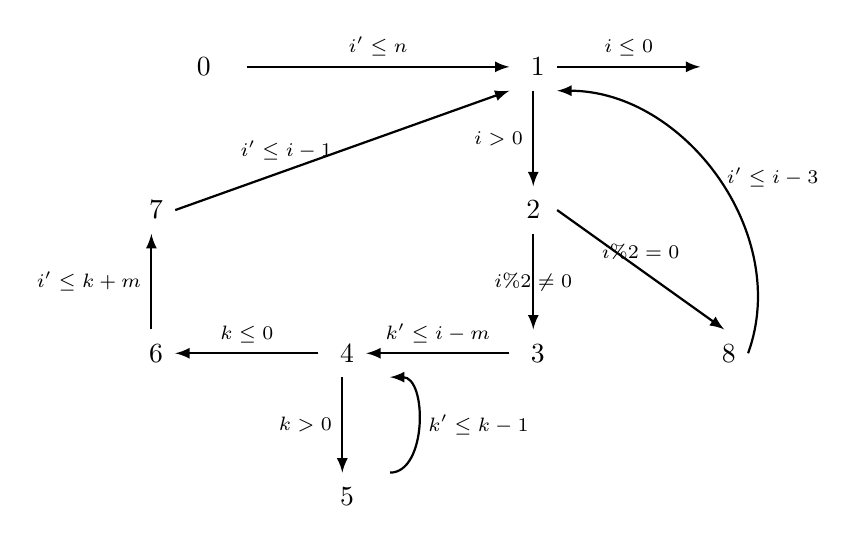
\begin{tikzpicture}[scale=\textwidth/20cm,samples=200]
  \draw[] (-7, 10) circle (0pt) node{{ $0$}};
  \draw[] (0, 10) circle (0pt) node{{ $1$}};
  \draw[] (0, 7) circle (0pt) node{\textbf{$2$}};
  \draw[] (0, 4) circle (0pt) node{{ $3$}};
  \draw[] (-4, 4) circle (0pt) node{{ $4$}};
  \draw[] (-8, 4) circle (0pt) node{{ $6$}};
  \draw[] (-4, 1) circle (0pt) node{{ $5$}};
  \draw[] (4, 4) circle (0pt) node{{ $8$}};
  \draw[] (-8, 7) circle (0pt) node{{ $7$}};
  % Counter Variables
  \draw[] (4.5, 10) circle (0pt) node {\textbf{$\lex$}};
  % \draw[] (6, 4) circle (0pt) node {{ $ex$}};
  %
  % Control Flow Edges:
  \draw[ thick, -latex] (-6, 10)    -- node [above] {\scriptsize $i' \leq n$}(-0.5, 10);
  \draw[ thick, -latex] (0, 9.5)    -- node [left] {\scriptsize $i > 0$} (0, 7.5) ;
  \draw[ thick, -latex] (0.5, 7)    -- node [above] {\scriptsize $ i \% 2 = 0 $}  (4, 4.5);
  \draw[ thick, -latex] (4.5, 4)    to  [out=70,in=0]   node [right] {\scriptsize $i' \leq i - 3$ }(0.5, 9.5);
  \draw[ thick, -latex]  (0, 6.5)   -- node  {\scriptsize $i \% 2 \neq 0$}  (0, 4.5) ;
  \draw[ thick, -latex]  (-0.5, 4)  -- node [above] {\scriptsize $k' \leq i - m$ }  (-3.5, 4) ;
  \draw[ thick, -latex]  (-4.5, 4)  -- node [above] {\scriptsize $k \leq 0$ }  (-7.5, 4);
  \draw[ thick, -latex] (0.5, 10)   -- node [above] {\scriptsize $i \leq 0$}  (3.5, 10);
  \draw[ thick, -latex] (-4, 3.5)   -- node [left] {\scriptsize $k > 0$}  (-4, 1.5);
  \draw[ thick, -latex] (-3, 1.5)   to  [out=0,in=0] node [right] {\scriptsize $k' \leq k- 1$}  (-3, 3.5);
  \draw[ thick, -latex] (-8, 4.5)   --  node [left] {\scriptsize $i' \leq k + m$ }(-8, 6.5);
  \draw[ thick, -latex] (-7.5, 7)  --  node [left] {\scriptsize $i' \leq i - 1$ }(-0.5, 9.5);
  % \draw[ thick, -latex] (6, 6.5)  -- node [right] {$\top$} (6, 4.5) ;
  \end{tikzpicture}
  \caption{}
    \end{centering}
    \end{subfigure}
\begin{subfigure}{.9\textwidth}    
\begin{centering}
  {\small
  $\tpath_0 = (0 \to 1)$
  \quad
  $\tpath_1 = (1 \to 2 \to 3 \to 4)$
  \quad
  $\tpath_2 = (4 \to 6 \to 7 \to 1)$
  \quad
  $\tpath_3 = (4 \to 5 \to 4)$
  \quad
  $\tpath_4 = (1 \to 2 \to 8 \to 1)$
  \quad
  $\tpath_5 = (1 \to \lex)$
  \\
  $
  \tpath_0 ; \rpchoose{ 1: \rprepeat(\tpath_1; 4:\rprepeat(\tpath_3); \tpath_2; \tpath_4), 
  1: \rprepeat(\tpath_4; \tpath_1; 4:\rprepeat(\tpath_3); \tpath_2) }; \tpath_5
  $
  }
  % \caption{}
    \end{centering}
    \end{subfigure}
  \caption{
  (a) The program of the two paths loop with a nested Loop in one path,
    (b) The corresponding \emph{Abstract Transition Graph}, $\absG(\kw{nestedOdd}(n, m))$. }
      \label{fig:relatedNestedWhileOdd-overview}
  \end{figure}
  }
  %
  \end{example}    
  

\textbf{Challenge I}
The example program in Figure~\ref{fig:relatedNestedWhileOdd-overview}(a) has two level nested loops, outer loop $L_1$ and nested loop $L_4$ which is in the first path of $L_1$. Given $n \geq m \geq 0$,
the expected \emph{reachability-bound}s for locations in outer loop $3, 6, 7$ and $8$ are all $\lfloor\frac{m}{4}\rfloor$,
% for $8$ is $\lfloor\frac{m}{4}\rfloor + 1$,
for location $2$ is $\lfloor\frac{m}{2}\rfloor$ and $\lfloor\frac{m}{2}\rfloor + 1$ for location $1$.
{Though within the same loop $L_1$, the bounds for different locations are different.}
Amortized analysis tools such as Loopus~\cite{SinnZV17}, KoAT~\cite{BrockschmidtEFFG14,FalkeKS12,FalkeKS11}, C4B~\cite{CarbonneauxHS15}, etc. ignore path sensitivity and approximate the bound $n$ as the bound for loop $L_1$. 
While some path-refinement-based methods such as \cite{GulwaniZ10,GulwaniJK09}, CoFloCo~\cite{Montoya17,Flores-Montoya16,Flores-MontoyaH14} and etc. give the same bound for all the locations within the loop $L_1$. 
Although we can reuse their results i.e., loop bounds as the \emph{reachability-bound} for location $1$ and $2$,
it is still unclear for locations $3, 6, 7$, and $8$.
%
This motivates our first key novelty -- the \emph{path reachability-bound}
for a loop-free and interleaving-free path $\tpath$.
It bounds the times that each path is evaluated in a path-refined program.

\textbf{Challenge II} T
\highlight{he second challenge occurs in the nested loop.
In the command of label 3, $k$ is reset by $i - m$, and $i$ is reset by $k + m$ after the
loop $L_4$, so $L_4$ is only executed in the first iteration of loop $L_1$.
We say the loop $L_4$ is ``reached'' only once in the outer loop $L_1$.
% \\
The total number of loop iterations is
$n - m + \lfloor\frac{m}{2}\rfloor + 1$,
and the tight \emph{reachability-bound} for location $5$ inside $L_4$ is $m$, which is the same as this innermost loop iteration bound.
% \\
}
Existing approaches either ignore path sensitivity or compute the same bound for all the locations in a loop.
None of them can give the precise \emph{reachability-bound}s for different locations in the loop.
Even if the loop bound is known, they are non-trivial to compute.
This motivates us to consider our second novel quantity --
the numbers of iterations of the {outer loop $L_1$} such that,
during these iterations, the loop $L_4$ is ``entered'', which is expected to be $1$. 
We refer to this quantity as the \emph{loop reachability} of the inner loop $L_4$ w.r.t the outer loop $L_1$.
% of the location within loop $L_6$ w.r.t the loops $L_3$ and $L_1$.
By multiplying the \emph{path reachability-bound} of $\tpath_3$ within $L_4$
with its \emph{loop reachability-bound} w.r.t $L_1$, we can obtain an accurate
\emph{reachability-bound} for location $5$.
% This quantity isn't considered or computed in any of the previous works.
\cite{GulwaniJK09} considers a similar quantity using the \emph{Progress Invariant}, but it bounds the iteration times of {inner loop $L_4$} w.r.t. one iteration of $L_1$, which is $m$. They still over-approximate the bound for locations inside $L_4$ as $m \times (n - m)$.
With these two key quantities, our algorithm computes the reachability-bound for this example through the following steps.
